\documentclass{standalone}
\begin{document}
\section{Multidimensional advection scheme}

The advection of a dependent variable $\phi$ is given by the flux form conservation equation:
\begin{align}
	\frac{\partial \phi}{\partial t} + \nabla \cdot \left( \bm{u} \phi \right) = 0 \label{eqn:advection}
\end{align}
where $\bm{u}$ is a prescribed wind field.  The time derivative is discretised using a three-stage, second-order Runge-Kutta scheme:
\begin{subequations}
\begin{align}
	\phi^\star &= \phi^{(n)} + \Delta t f(\phi^{(n)}) \\
	\phi^{\star\star} &= \phi^{(n)} + \frac{\Delta t}{2} \left( f(\phi^{(n)}) + f(\phi^\star) \right) \\
	\phi^{(n+1)} &= \phi^{(n)} + \frac{\Delta t}{2} \left( f(\phi^{(n)}) + f(\phi^{\star\star}) \right)
\end{align}
\end{subequations}
where \(f(\phi^{(n)}) = - \nabla \cdot (\bm{u} \phi^{(n)})\) at time level \(n\).

Using the finite volume method, the wind field is prescribed at face centroids and the dependent variable is stored at cell centroids.  The divergence term in equation~\eqref{eqn:advection} is discretised using Gauss's theorem:
\begin{align}
	\nabla \cdot \left( \bm{u} \phi \right) \approx \frac{1}{\mathcal{V}_c} \sum_{f \in c} \bm{u}_f \cdot \bm{S}_f \phi_F
\end{align}
where $\mathcal{V}_c$ is the cell volume, $\bm{u}_f$ is a wind vector prescribed at a face, ${\bm{S}_f}$ is the surface area vector with a direction outward normal to the face and a magnitude equal to the face area, and $\sum_{f \in c}$ denotes a summation over all faces $f$ belonging to cell $c$.  The value of the dependent variable at the face, $\phi_F$, is approximated by a least squares fit over a stencil of surrounding cell centre values.

\begin{figure}
	\centering
	\includegraphics[width=4in]{interiorQuadStencil.png}
	\caption{\TODO{interior quad stencil}}
	\label{fig:interiorQuadStencil}
\end{figure}

To introduce the approximation method, we will consider how an approximate value is calculated for a face in the interior of a two-dimensional uniform quadrilateral mesh.  For any mesh, every interior face connects two adjacent cells.  The wind direction at the face determines which of the two adjacent cells is the upwind cell.  Since the stencil is upwind-biased, two stencils must be constructed for every interior face, and the appropriate stencil is chosen for each face depending on the wind direction at that face for every timestep.

The upwind-biased stencil for a face $f$ is shown in figure~\ref{fig:interiorQuadStencil}.  The wind at the face, $\bm{U}_f$, is blowing from the upwind cell $c_u$ to the downwind cell $c_d$.
To obtain an approximate value at $f$, a polynomial least squares fit is calculated using the stencil values.
The stencil has \num{4} points in $x$ and \num{3} points in $y$, leading to a natural choice of polynomial that is cubic in $x$ and quadratic in $y$:
\begin{align}
	\phi = a_1 + a_2 x + a_3 y + a_4 x^2 + a_5 xy + a_6 y^2 + a_7 x^3 + a_8 x^2 y + a_9 x y^2
\end{align}
A least squares approach is needed because the system of equations is overdetermined, with \num{12} stencil values but only \num{9} polynomial terms.  If the stencil geometry is expressed in a local coordinate system with the face centroid as the origin, then the approximated value $\phi_F$ is equal to the constant term $a_1$.

The remainder of this section generalises the the approximation technique for arbitrary meshes, explaining the methods for constructing stencils, choosing the terms of the polynomial, and ensuring numerical stability of the advection scheme.

\subsection{Stencil construction}

\subsection{Polynomial generation}
% generating candidates
% full rank check

\subsection{Stabilisation procedure}
% stability constraints
% reweighting

Stability constriants:
\begin{align}
	0.5 \leq u \leq 1 \\
	0 \leq d \leq 0.5 \\
	u - d \geq \max(|p|)
\end{align}

\begin{figure}
	\includegraphics[width=\textwidth]{stencilConstruction.png}
	\caption{\TODO{example stencils in interior of quad and hex meshes, and example stencil near boundary of a slanted cell mesh (taken from one of the test cases)}}
\end{figure}
\end{document}
